
    \documentclass{standalone}
\usepackage{tkz-fct}
\usepackage{tkz-euclide}
\usepackage{color}
\usepackage{amsmath}
\renewcommand*\familydefault{\sfdefault}
\usepackage{sansmath}
\sansmath
\definecolor{gray75}{gray}{0.75}
\begin{document}
 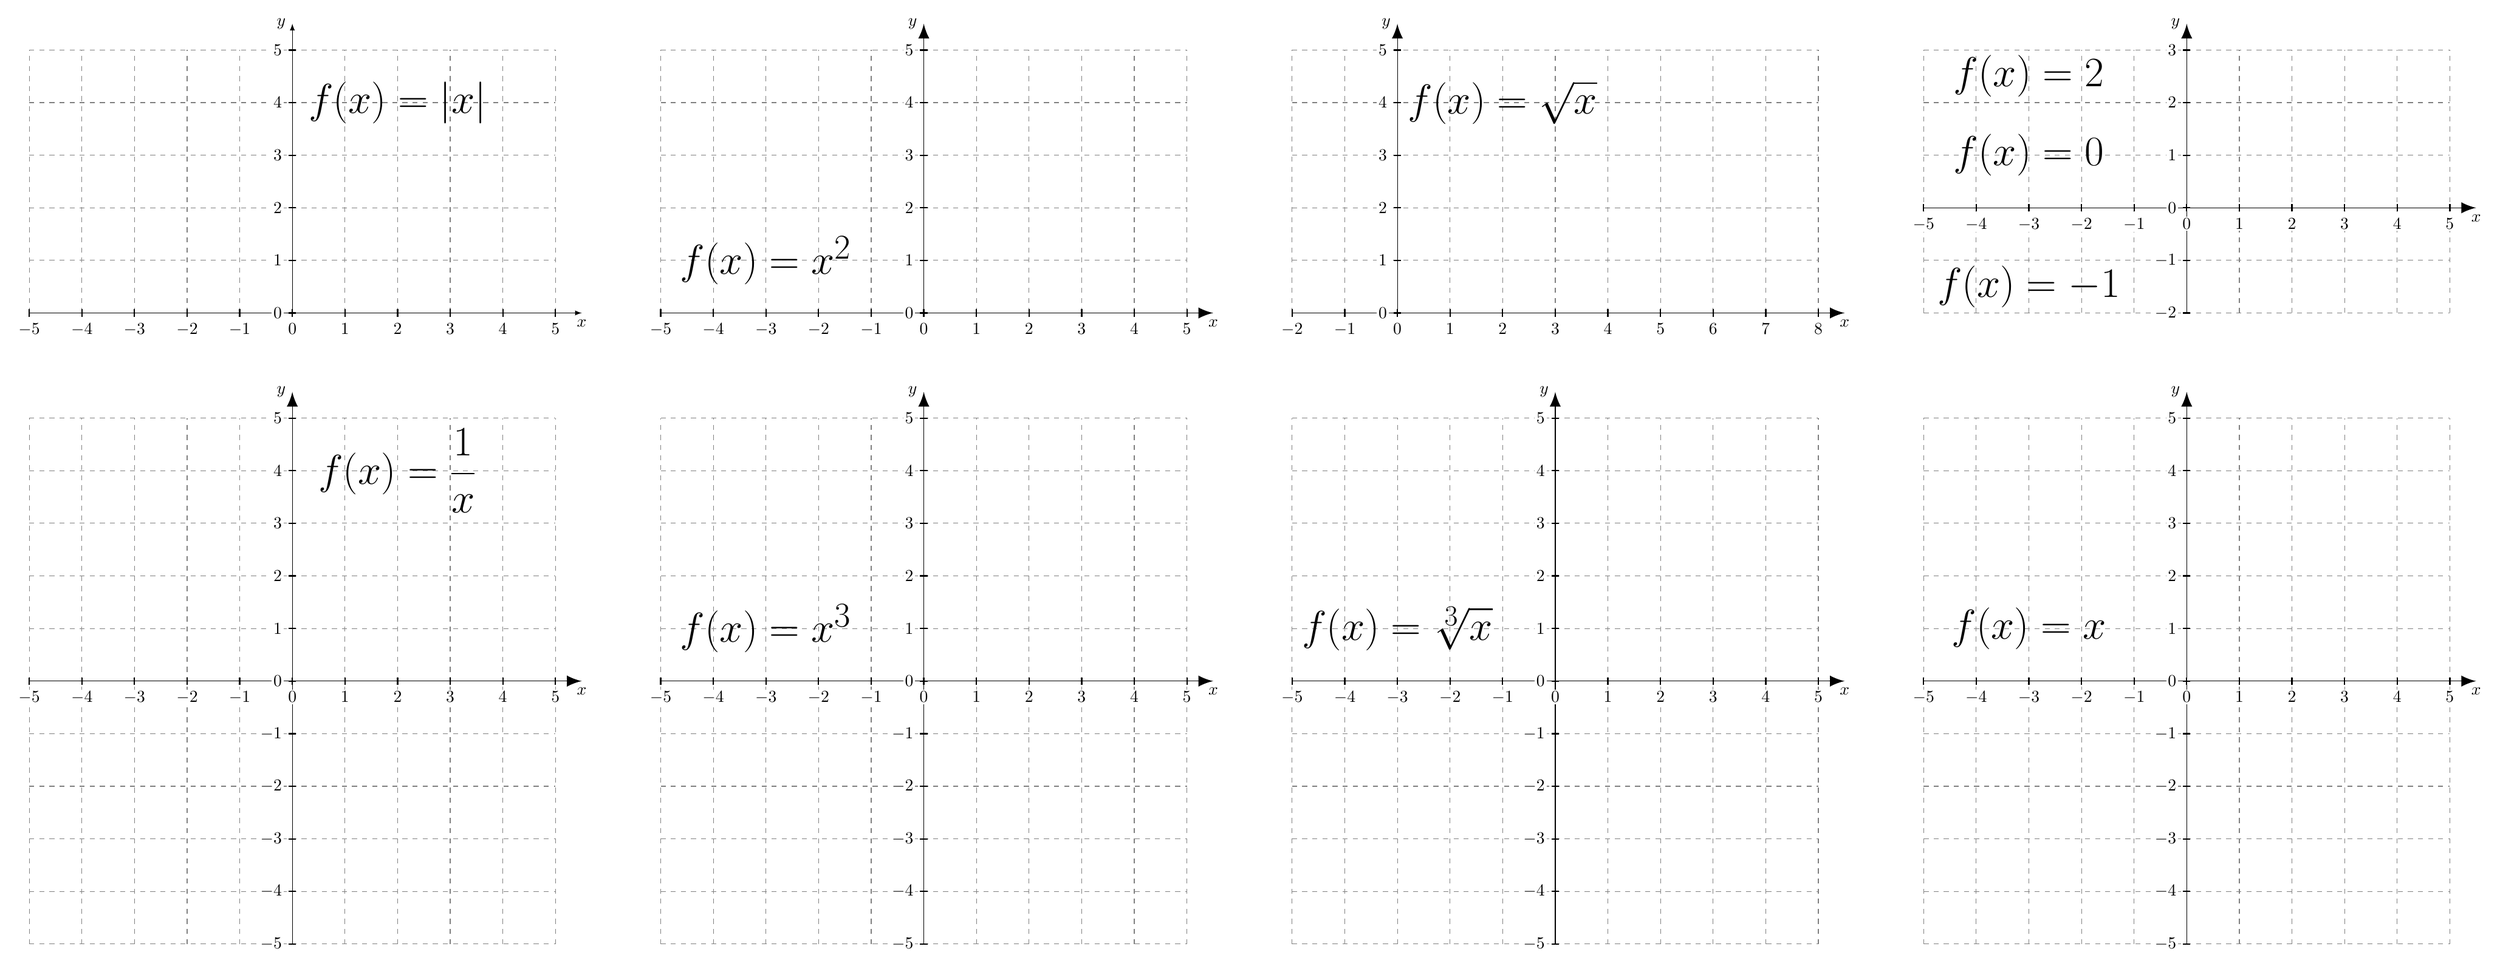
\begin{tikzpicture}[scale=1.1]
   \tkzInit[xmax=5.0,ymax=5.0,xmin=-5.0 ,ymin=0.0]
   \begin{scope}[dashed]
     \tkzGrid
   \end{scope}
   \tkzDrawX[label={$x$}]
   \tkzDrawY[label={$y$}]
   \tkzLabelX
   \tkzLabelY
   \tkzFct[line width=2pt,domain=-5:5]{(abs(x))}


   \tkzText(2,4){\Huge$f(x)=|x|$}
   \begin{scope}[xshift=12cm]
\tkzInit[xmax=5.0,ymax=5.0,xmin=-5.0 ,ymin=0.0]
   \begin{scope}[dashed]
     \tkzGrid
   \end{scope}
   \tkzDrawX[label={$x$}]
   \tkzDrawY[label={$y$}]
   \tkzLabelX
   \tkzLabelY
   \tkzFct[line width=2pt,domain=-2.5:2.5]{(x**2)}
   \tkzText(-3,1){\Huge$f(x)=x^{2}$}
\end{scope}
\begin{scope}[xshift=21cm]
  \tkzInit[xmax=8.0,ymax=5.0,xmin=-2.0 ,ymin=0.0]
   \begin{scope}[dashed]
     \tkzGrid
   \end{scope}
   \tkzDrawX[label={$x$}]
   \tkzDrawY[label={$y$}]
   \tkzLabelX
   \tkzLabelY
   \tkzFct[line width=2pt,domain=0:8]{(x**(0.5))}
   \tkzText(2,4){\Huge$f(x)=\sqrt{x}$}
\end{scope}
\begin{scope}[xshift=36cm, yshift=2cm]
   \tkzInit[xmax=5.0,ymax=3.0,xmin=-5.0 ,ymin=-2.0]
   \begin{scope}[dashed]
     \tkzGrid
   \end{scope}
   \tkzDrawX[label={$x$}]
   \tkzDrawY[label={$y$}]
   \tkzLabelX
   \tkzLabelY
   \tkzFct[line width=2pt,domain=-5:5]{(2)}
   \tkzFct[line width=2pt,domain=-5:5]{(0)}
   \tkzFct[line width=2pt,domain=-5:5]{(-1)}
   \tkzText(-3,2.5){\Huge$f(x)=2$}
   \tkzText(-3,1){\Huge$f(x)=0$}
   \tkzText(-3,-1.5){\Huge$f(x)=-1$}
 \end{scope}
 \begin{scope}[xshift=24cm, yshift=-7cm]
   \tkzInit[xmax=5.0,ymax=5.0,xmin=-5.0 ,ymin=-5.0]
   \begin{scope}[dashed]
     \tkzGrid
   \end{scope}
   \tkzDrawX[label={$x$}]
   \tkzDrawY[label={$y$}]
   \tkzLabelX
   \tkzLabelY
   \tkzFct[line width=2pt,domain=0:5]{(x**(1/3.0))}
   \tkzFct[line width=2pt,domain=-5:-0.000001]{(-1*abs(x)**(1/3.0))}
   \tkzText(-3,1){\Huge$f(x)=\sqrt[3]{x}$}
 \end{scope}
 \begin{scope}[yshift = -7cm]
   \tkzInit[xmax=5.0,ymax=5.0,xmin=-5.0 ,ymin=-5.0]
   \begin{scope}[dashed]
     \tkzGrid
   \end{scope}
   \tkzDrawX[label={$x$}]
   \tkzDrawY[label={$y$}]
   \tkzLabelX
   \tkzLabelY
   \tkzFct[line width=2pt,domain=-5:-0.1]{(1/x)}
   \tkzFct[line width=2pt,domain=0.1:5]{(1/x)}
   \tkzText(2,4){\Huge$f(x)=\dfrac{1}{x}$}

\end{scope}
\begin{scope}[xshift=12cm,yshift = -7cm]
   \tkzInit[xmax=5.0,ymax=5.0,xmin=-5.0 ,ymin=-5.0]
   \begin{scope}[dashed]
     \tkzGrid
   \end{scope}
   \tkzDrawX[label={$x$}]
   \tkzDrawY[label={$y$}]
   \tkzLabelX
   \tkzLabelY
   \tkzFct[line width=2pt,domain=0:2.5]{(x**3)}
   \tkzFct[line width=2pt,domain=-2.5:0]{(-1*abs(x)**3)}
   \tkzText(-3,1){\Huge$f(x)=x^{3}$}
\end{scope}
\begin{scope}[xshift=36cm,yshift=-7cm]
   \tkzInit[xmax=5.0,ymax=5.0,xmin=-5.0 ,ymin=-5.0]
   \begin{scope}[dashed]
     \tkzGrid
   \end{scope}
   \tkzDrawX[label={$x$}]
   \tkzDrawY[label={$y$}]
   \tkzLabelX
   \tkzLabelY
   \tkzFct[line width=2pt,domain=-5:5]{(x)}
   \tkzText(-3,1){\Huge$f(x)=x$}
\end{scope}

\end{tikzpicture}
\end{document}
